\section{Gravity waves}

Gravity waves test taken from Weller and Shahrokhi.

\begin{itemize}
\item Reproduced result for BTF from W\&S
\item Vertical mixing at ground in lee of orography seen in results for snapCol and snap meshes.  This occurs in the lowest two rows of the mesh: lower layer $\theta$ is warmer, next layer above is cooler.  Feature is visible after t=3600s (Figure~\ref{fig:gw:mixing-3600s}), becomes more pronounced by t=18000s (Figure~\ref{fig:gw:mixing-18000s}).
\end{itemize}

\subsection{Investigation of vertical mixing}
Initially suspected mixing was due to computation mode of Lorenz vertical staggering but now it seems not:
\begin{itemize}
	\item plot UfDiff as a vector field doesn't seem to show any velocity anomalies in BTF or snalCol (Figure~\ref{fig:gw:ufdiff})
	\item plot of $\theta$ field shows that mixing is not strong enough to overcome stratification (Figure~\ref{fig:gw:theta})
	\item doubling mountain height causes mixing to appear in BTF case, and increases to three rows of mixing in SnapCol (Figure~\ref{fig:gw:double-height})
\end{itemize}

\begin{figure}
	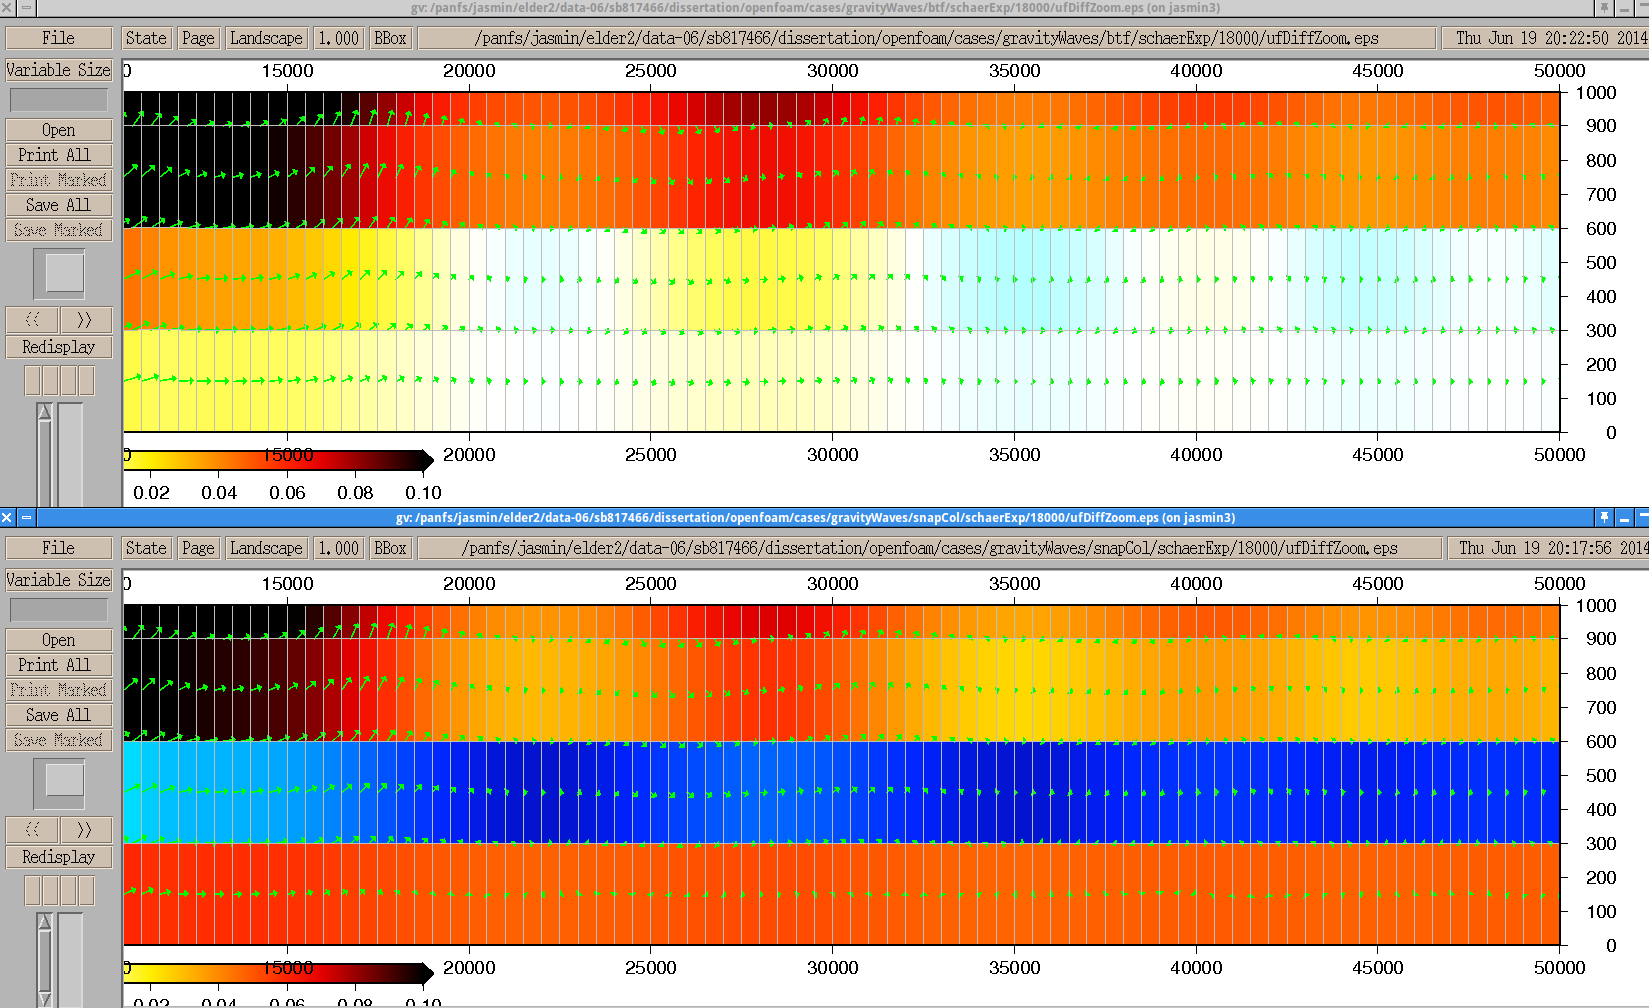
\includegraphics[width=\textwidth]{interim-results/gravityWavesBTFSnapColVelocityVectors.png}
	\caption{UfDiff after t=18000s, BTF and SnapCol meshes}
	\label{fig:gw:ufdiff}
\end{figure}

\begin{figure}
	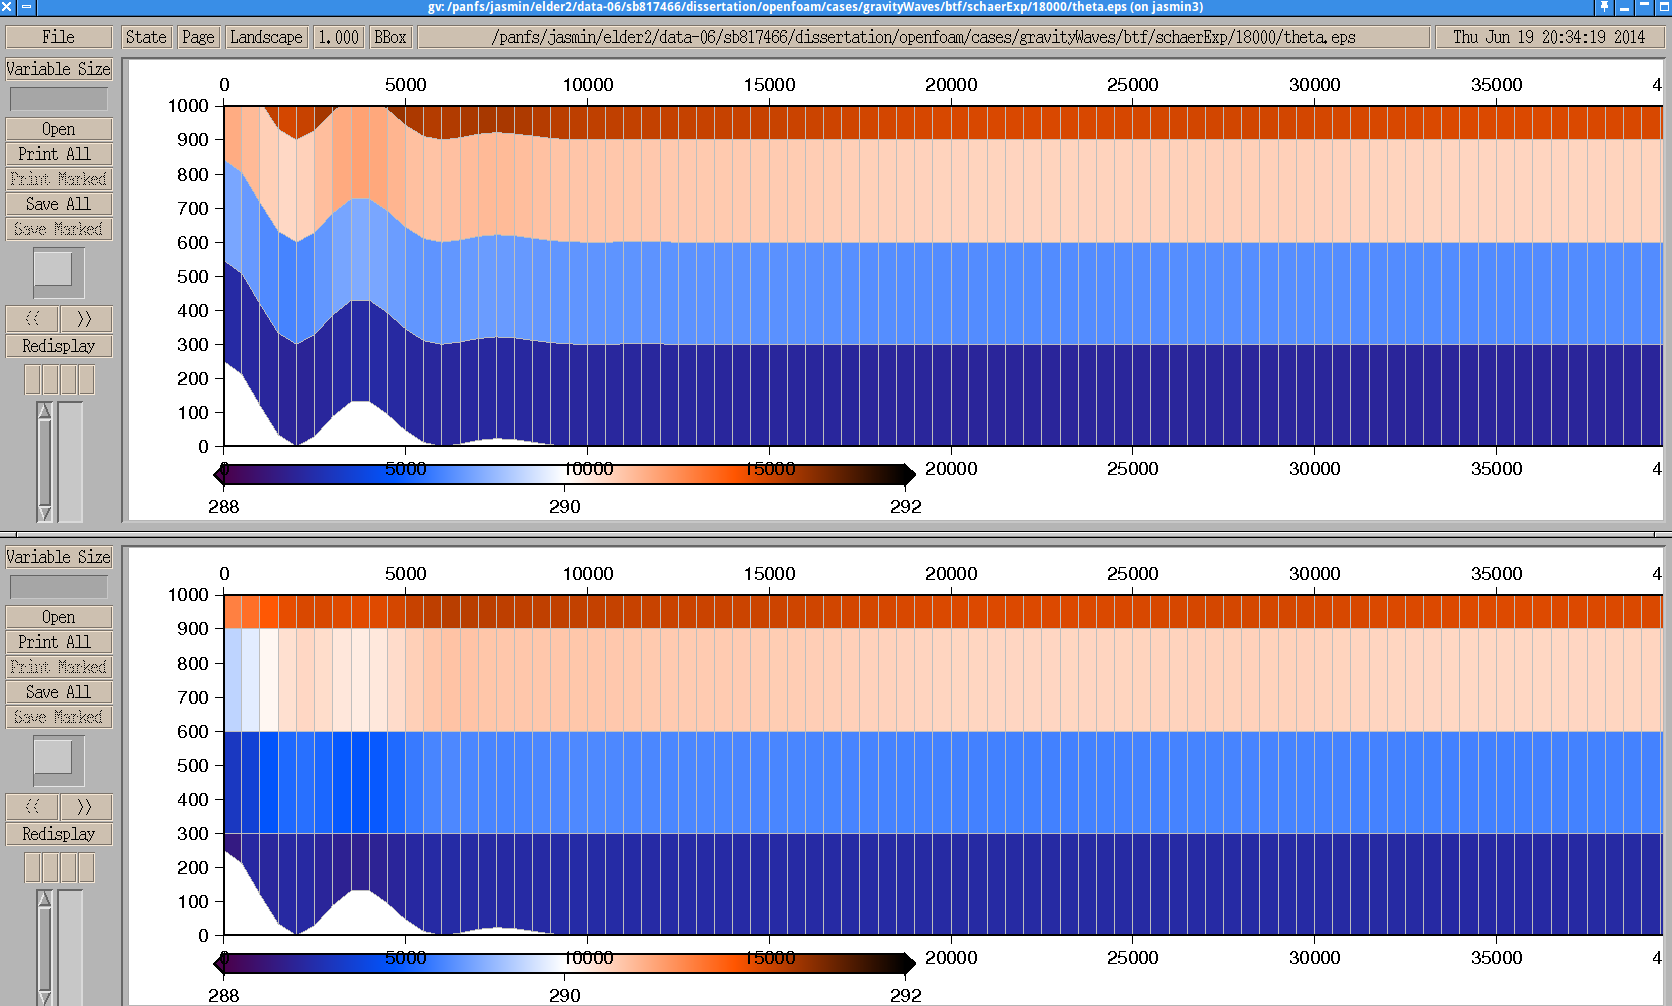
\includegraphics[width=\textwidth]{interim-results/gravityWavesBTFSnapColTheta.png}
	\caption{$\theta$ after t=18000s, BTF and SnapCol meshes}
	\label{fig:gw:theta}
\end{figure}

\begin{figure}
	BTF
	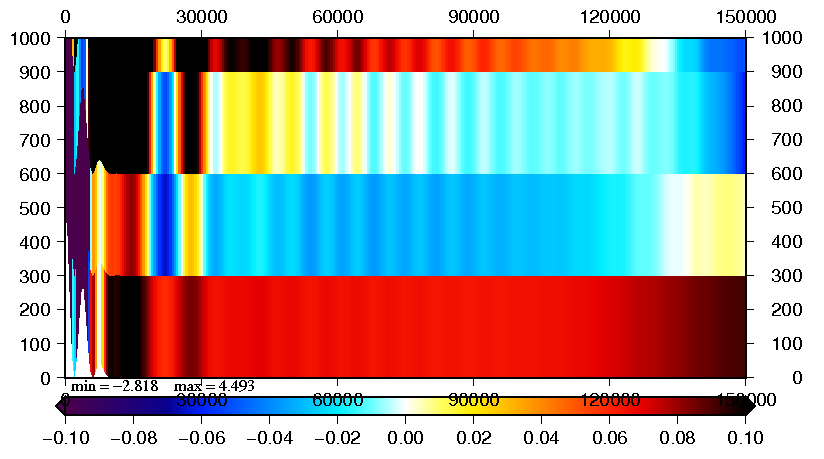
\includegraphics[width=\textwidth]{interim-results/gravityWavesBTFDoubleHeightThetaDiffZoom.png}
	SnapCol
	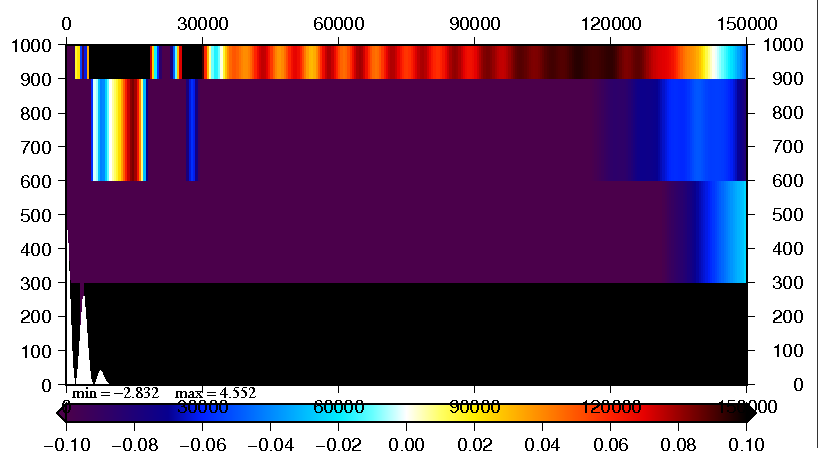
\includegraphics[width=\textwidth]{interim-results/gravityWavesSnapColDoubleHeightThetaDiffZoom.png}

	\caption{double height mountain, thetaDiff after t=18000s}
	\label{fig:gw:double-height}
\end{figure}

To see if the computational mode is present in more than one test case, try:
\begin{itemize}
\item halving $\Delta z$ --- are 2 rows of cells still affected (suggests computational mode), or 4 rows (physical problem?)
\item change stability (zN in environmentalProperties)
\end{itemize}

\begin{figure}
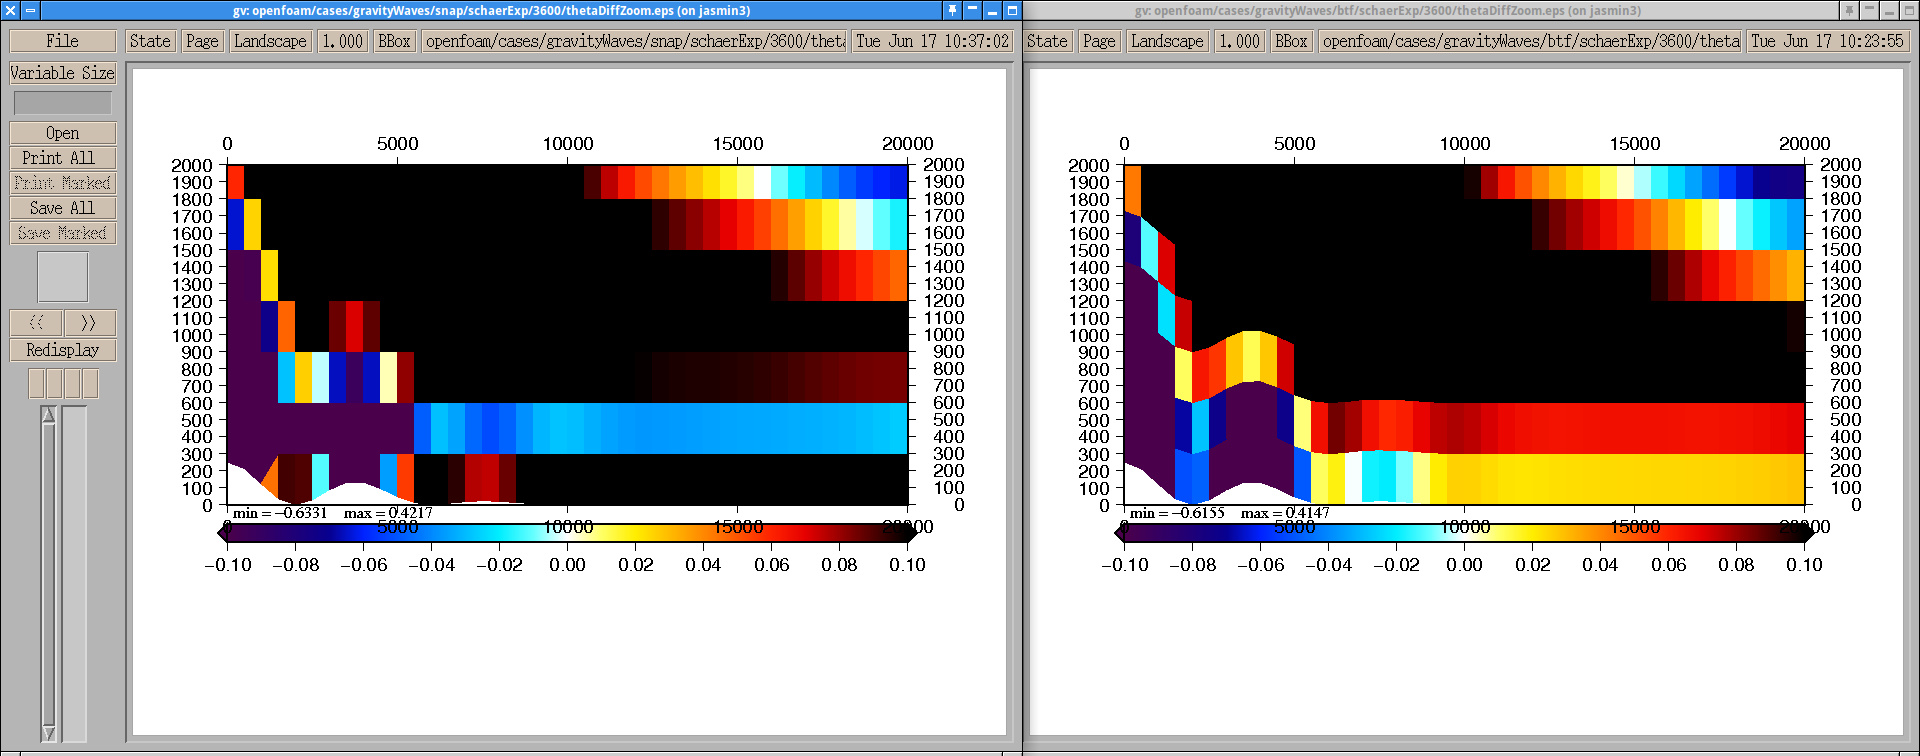
\includegraphics[width=\textwidth]{interim-results/gravityWavesBTFsnapMidZoom3600.png}
\caption{Vertical mixing after t=3600s, snap mesh left, BTF right}
\label{fig:gw:mixing-3600s}
\end{figure}

\begin{figure}
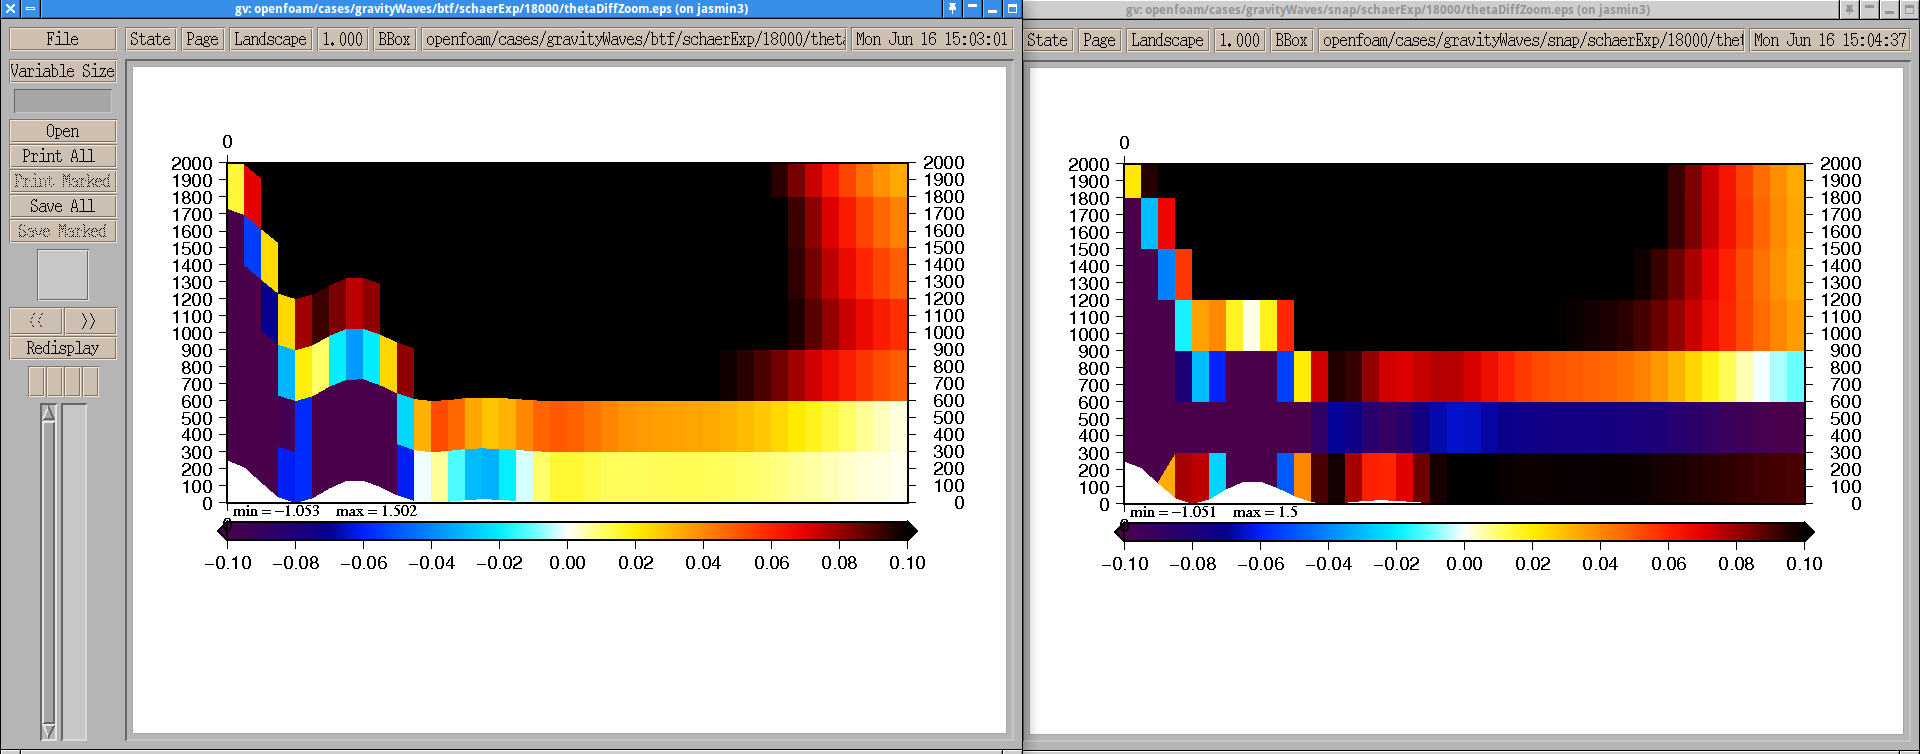
\includegraphics[width=\textwidth]{interim-results/gravityWavesBTFsnapMidZoom18000.png}
\caption{Vertical mixing after t=18000s.  Confusingly, snap mesh right, BTF left!}
\label{fig:gw:mixing-18000s}
\end{figure}
